\documentclass[12pt,a4paper]{article}
\usepackage[utf8]{inputenc}
\usepackage[english]{babel}

\usepackage{amsmath}
\usepackage{amsfonts}
\usepackage{amssymb}

\usepackage{graphicx}
\usepackage{lmodern}
\usepackage{tikz}
\usepackage{titlesec}
\usepackage{environ}
\usepackage{xcolor}
\usepackage{fancyhdr}
\usepackage[colorlinks = true, linkcolor = black]{hyperref}
\usepackage{xparse}
\usepackage{enumitem}
\usepackage{comment}
\usepackage{wrapfig}

\usepackage[left=2cm,right=2cm,top=2cm,bottom=2cm]{geometry}
\usepackage{multicol}
\usepackage[indent=0pt]{parskip}

\newcommand{\spaceP}{\vspace*{0.5cm}}
\newcommand{\Span}{\mathrm{Span}\,}
\newcommand{\range}{\mathrm{range}\,}
\newcommand{\ra}{\rightarrow}

%% Redefining sections
\newcommand{\sectionformat}[1]{%
    \begin{tikzpicture}[baseline=(title.base)]
        \node[rectangle, draw] (title) {#1};
    \end{tikzpicture}
    
    \noindent\hrulefill
}

% default values copied from titlesec documentation page 23
% parameters of \titleformat command are explained on page 4
\titleformat%
    {\section}% <command> is the sectioning command to be redefined, i. e., \part, \chapter, \section, \subsection, \subsubsection, \paragraph or \subparagraph.
    {\normalfont\large\scshape}% <format>
    {}% <label> the number
    {0em}% <sep> length. horizontal separation between label and title body
    {\centering\sectionformat}% code preceding the title body  (title body is taken as argument)

%% Set counters for sections to none
\setcounter{secnumdepth}{0}

%% Set the footer/headers
\pagestyle{fancy}
\fancyhf{}
\renewcommand{\headrulewidth}{0pt}
\renewcommand{\footrulewidth}{2pt}
\lfoot{P.-O. Paris{\'e}}
\cfoot{MATH 302}
\rfoot{Page \thepage}

%% Defining example environment
\newcounter{example}[section]
\NewEnviron{example}%
	{%
	\noindent\refstepcounter{example}\fcolorbox{gray!40}{gray!40}{\textsc{\textcolor{red}{Example~\theexample.}}}%
	%\fcolorbox{black}{white}%
		{  %\parbox{0.95\textwidth}%
			{
			\BODY
			}%
		}%
	}

% Theorem environment
\NewEnviron{theorem}%
	{%
	\noindent\refstepcounter{example}\fcolorbox{gray!40}{gray!40}{\textsc{\textcolor{blue}{Theorem~\theexample.}}}%
	%\fcolorbox{black}{white}%
		{  %\parbox{0.95\textwidth}%
			{
			\BODY
			}%
		}%
	}

\NewEnviron{notes}%
	{%
	\noindent \fcolorbox{gray!40}{gray!40}{\textsc{\textcolor{blue}{Solution.}}}%
	%\fcolorbox{black}{white}%
		{  %\parbox{0.95\textwidth}%
			{
			\textcolor{blue}{%
			\BODY
			}
			}%
		}%
	}
%%% Ignorer les notes
\excludecomment{notes}

%%%%
\begin{document}
\thispagestyle{empty}

\begin{center}
\vspace*{2.5cm}

{\Huge \textsc{Math 302}}

\vspace*{2cm}

{\LARGE \textsc{Chapter 6}} 

\vspace*{0.75cm}

\noindent\textsc{Section 6.1 and 6.2: Spring-mass System}

\vspace*{0.75cm}

\tableofcontents

\vfill

\noindent \textsc{Created by: Pierre-Olivier Paris{\'e}} \\
\textsc{Fall 2022}
\end{center}

\newpage

\section{Setup}

Consider an object with a mass $m$ suspended from a spring of negligible mass.
	\begin{itemize}
	\item When the object is at rest and the forces sum to zero, we say that the spring-mass system is in \textbf{equilibrium}.
	\item When the system is at equilibrium, we call the position of the object the \textbf{equilibrium position}.
	\item We let $y(t)$ be the position of the object with respect to the equilibrium position.
	\end{itemize}
	
\vspace*{20pt}

\begin{minipage}{0.5\textwidth}
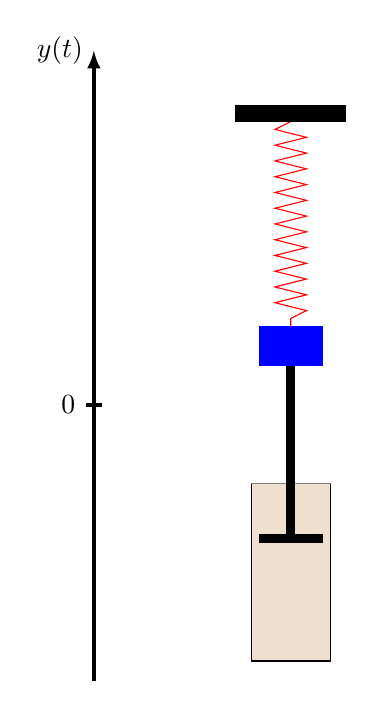
\begin{tikzpicture}
\draw[black, very thick, >=latex, ->] (0, -1) -- (0, 7)node[left]{$y(t)$};
\draw[black, very thick] (0.1, 2.5) -- (-0.1, 2.5)node[left]{$0$};
\draw[black!50, fill=brown!25] (2, -0.75) -- (3,-0.75) -- (3, 1.5) -- (2, 1.5) -- (2, -0.75);
\draw[black] (3, 1.5) -- (3, -0.75) -- (2, -0.75) -- (2, 1.5);
\draw[black, fill=black] (2.1, 0.75) -- (2.9, 0.75) -- (2.9, 0.85) -- (2.1, 0.85) -- (2.1, 0.75);
\draw[black, fill=black] (2.45, 0.85) -- (2.55, 0.85) -- (2.55, 3) -- (2.45, 3) -- (2.45, 0.85);
\draw[blue, fill=blue] (2.1, 3) -- (2.9, 3) -- (2.9, 3.5) -- (2.1, 3.5) -- (2.1, 3);
\draw[red] (2.5, 3.5) -- (2.5, 3.6) -- (2.7, 3.7) -- (2.3, 3.8) -- (2.7, 3.9) -- (2.3, 4) -- (2.7, 4.1) -- (2.3, 4.2) -- (2.7, 4.3) -- (2.3, 4.4) -- (2.7, 4.5) -- (2.3, 4.6) -- (2.7, 4.7) -- (2.3, 4.8) -- (2.7, 4.9) -- (2.3, 5) -- (2.7, 5.1) -- (2.3, 5.2) -- (2.7, 5.3) -- (2.3, 5.4) -- (2.7, 5.5) -- (2.3, 5.6) -- (2.7, 5.7) -- (2.3, 5.8) -- (2.7, 5.9) -- (2.3, 6) -- (2.5, 6.1);
\draw[black, fill=black] (1.8, 6.1) -- (3.2, 6.1) -- (3.2, 6.3) -- (1.8, 6.3) -- (1.8, 6.1);
\end{tikzpicture}

\textsc{Figure}: Illustration of the spring-mass system with damping.
\end{minipage}
\begin{minipage}{0.5\textwidth}
\vspace*{4cm}
\end{minipage}


\vspace*{16pt}
	
	
From Newton's second Law, we have
	\begin{align*}
	m y'' = \phantom{-mg + F_d + F_s + F = -mg - cy' + F_s + F .}
	\end{align*}
The force $F_s$ is related to $y$ by
	\begin{align*}
	F_s = mg - k y .
	\end{align*}		
	
Substituting this expression of $F_s$ in the expression of $my''$, we obtain the following ODE called the \textbf{equation of motion}:
	\begin{align*}
	my'' + cy' + ky = F .
	\end{align*}

\newpage

\section{Simple Harmonic Motion}
We'll consider no exterior force and no damping. Therefore, the ODE becomes
	\begin{align*}
	my'' + ky = 0 \iff y'' + (k/m) y = 0 .
	\end{align*}
The solution is therefore given by
	\begin{align*}
	y(t) = c_1 \cos \big( t \sqrt{\frac{k}{m}} \big) + c_2 \sin \big( t \sqrt{\frac{k}{m}} \big) .
	\end{align*}
	
	\underline{Remark:}
	\begin{itemize}
	\item An important quantity is $\Delta l$, the difference between the natural length of a spring and it's length at the equilibrium. We have
		\begin{align*}
		mg = k \Delta l \iff \frac{k}{m} = \frac{g}{\Delta l} .
		\end{align*}
	\end{itemize}
	
Using some trigonometry identities, we can rewrite the solution as
	\begin{align*}
	y(t) = R \cos \Big( t \sqrt{\frac{k}{m}} - \phi \Big)
	\end{align*}
where $R$ and $\phi$ are constants related to $c_1$ and $c_2$ in the following way:
	\begin{align*}
	c_1 = R\cos \phi \quad \text{ and } \quad c_2 =  R \sin \phi .
	\end{align*}
	
	
	\begin{figure}[ht]
	\centering
	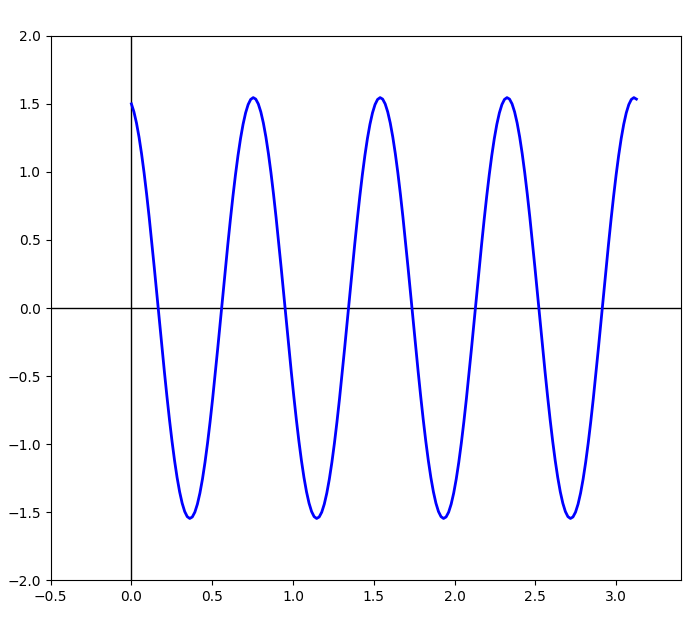
\includegraphics[scale=0.4]{fig1.png}
	\caption{Example of a harmonic motion: $y(t) = (3/2) \cos (8t) - (3/8) \sin (8t)$ or $y(t) = (3\sqrt{17}/8) \cos (8t + 0.245)$. See Example 6.1.1, page 269 and Example 6.1.2, page 272.}
	\end{figure}


	
	
\begin{notes}
\begin{example}
An object stretches a spring $6$cm in equilibrium.
\begin{enumerate}[label=\textbf{(\alph*)}]
\item Set up the equation of motion and find its general solution.
\item Find the displacement of the object for $t > 0$ if it has initially displaced 18 inches above the equillibrium and given a downward velocity of 3ft/s.
\end{enumerate}
\end{example}
\end{notes}


\newpage

\section{Undamped Forced Oscillation}
We now consider an external force $F$ of the form
	\begin{align*}
	F(t) = F_0 \cos (\omega t ) .
	\end{align*}
So, we want to solve
	\begin{align*}
	y'' + (k/m) y = \frac{F_0}{m} \cos (\omega t) .
	\end{align*}

Two cases:
	\begin{itemize}
	\item If $\omega \neq \sqrt{k/m}$, then the solution is periodic and do not blow up!
	\item If $\omega = \sqrt{k/m}$, then the solution blows up!
	\end{itemize}

To simplify the notation, we use the following notation:
	\begin{align*}
	\omega_0 := \sqrt{k}{m} .
	\end{align*}
	
\subsection{First case: $\omega_0 \neq \omega$}
The solution is
	\begin{align*}
	y(t) = c_1 \cos (\omega_0 t) + c_2 \sin (\omega_0 t) + \frac{F_0}{m (\omega_0^2 - \omega^2 )} \sin (\omega t) .
	\end{align*}
If we suppose that $y(0) = 0$ and $y'(0) = 0$, then from some clever tricks and trig identities, we can simplify the expression of $y(t)$ to
	\begin{align*}
	y(t) &= \frac{2 F_0}{m (\omega_0^2 - \omega^2)} \sin \Big( \frac{[\omega_0 - \omega ] t}{2} \Big) \sin \Big( \frac{[\omega_0 + \omega] t}{2} \Big) \\
	&= R(t) \sin \Big( \frac{[\omega_0 + \omega ]t}{2} \Big) .
	\end{align*}

\underline{Remark:}
	\begin{itemize}
	\item The function $R(t)$ is called a \textbf{beat}.
	\end{itemize}

\begin{figure}
\centering
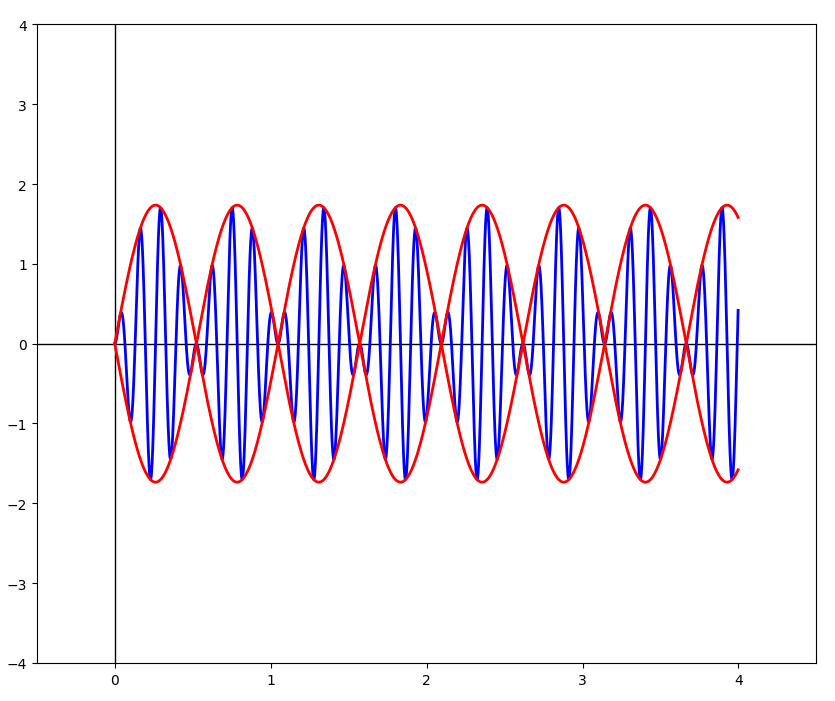
\includegraphics[scale=0.5]{fig2.png}
\caption{In blue: Solution with $F_0 = 4000$, $m = 4$, $\omega_0 = 54$ and $w = 42$. In red: the \textit{beat}.}
\end{figure}

\newpage

\subsection{Second case: $\omega_0 = \omega$}
The solution is
	\begin{align*}
	y(t) = c_1 \cos (\omega_0 t) + c_2 \sin (\omega_0 t) + \frac{F_0}{2m \omega_0} t \sin (\omega_0 t) .
	\end{align*}

We can show that the values of $y(t)$ oscillate between the lines
	\begin{align*}
	y = \frac{F_0}{2 m \omega_0} t \quad \text{ and } \quad y = - \frac{F_0}{2 m \omega_0} t .
	\end{align*}
	
\underline{Remark:}
	\begin{itemize}
	\item As $t \ra \infty$, we see that the oscillations of $y(t)$ become bigger and bigger.
	\item Such a phenomena is called \textbf{resonance}.
	\item A resonance may be dangerous for, amongs other examples, suspended bridges.
	\end{itemize}
	
	\begin{figure}[ht]
	\centering
	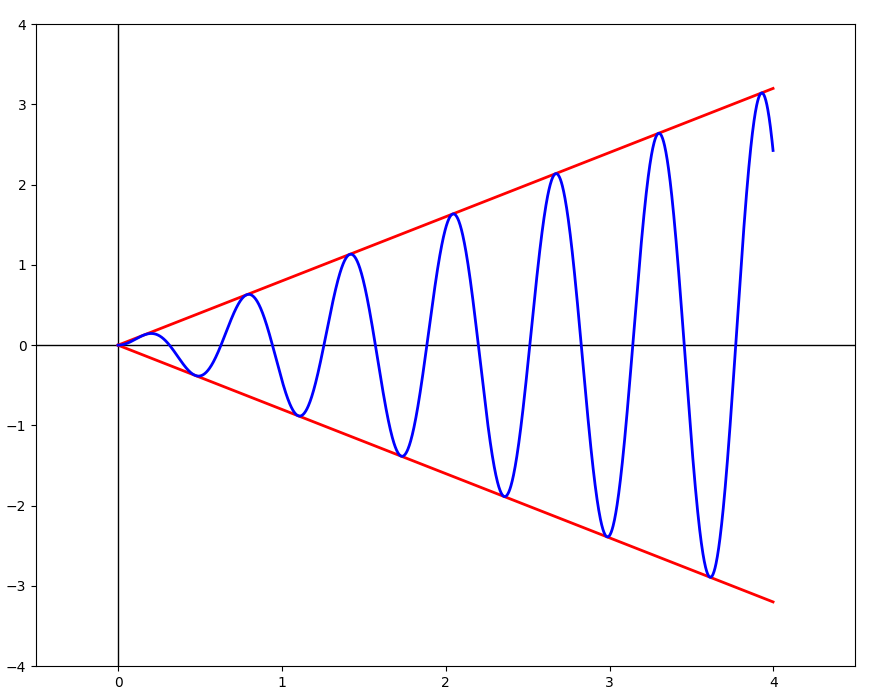
\includegraphics[scale=0.5]{fig3.png}
	\caption{In blue: Graph of the solution with $c_1 = 0$ and $c_2 = 0$ corresponding to $y(0) = y'(0) = 0$. In red: The shell containing the solution (maximum and minimum possible values).}
	\end{figure}
	
	\newpage
	
	\section{Free Vibrations With Damping}
	We consider the spring-mass system with $c \neq 0$. We therefore have
		\begin{align*}
		my'' + cy' + ky = 0 .
		\end{align*}
	The solutions will now depend on the roots of the characteristic polynomial:
		\begin{align*}
		r_1= \frac{-c - \sqrt{c^2 - 4mk}}{2m} \quad \text{ and } \quad r_2 = \frac{-c + \sqrt{c^2 - 4mk}}{2m} .
		\end{align*}
		
	\subsection{Underdamped Motion}
	\begin{itemize}
	\item The motion of the mass is said to be  \textbf{underdamped} if $c < \sqrt{4mk}$.
	
	\item If $\omega_1 = \frac{\sqrt{4mk - c^2}}{2m}$, then the expression of the roots become
		\begin{align*}
		r_1 = -\frac{c}{2m} - i \omega_1 \quad \text{ and } \quad r_2 = -\frac{c}{2m} + i \omega_1
		\end{align*}
	
	
	\item The general solution is therefore
		\begin{align*}
		y (t)= e^{-ct/2m} \big( c_1 \cos (\omega_1 t) + c_2 \sin (\omega_1 t) \big) .
		\end{align*}
	
	\item The expression of the solution can be simplified to% where $R = \sqrt{c_1^2 + c_2^2}$ and $\phi$ are parameters,
		\begin{align*}
		y(t) = R e^{-ct/2m} \cos \big( \omega_1 t - \phi \big) .
		\end{align*}
	
	\end{itemize}
	
	\begin{figure}[h]
	\centering
	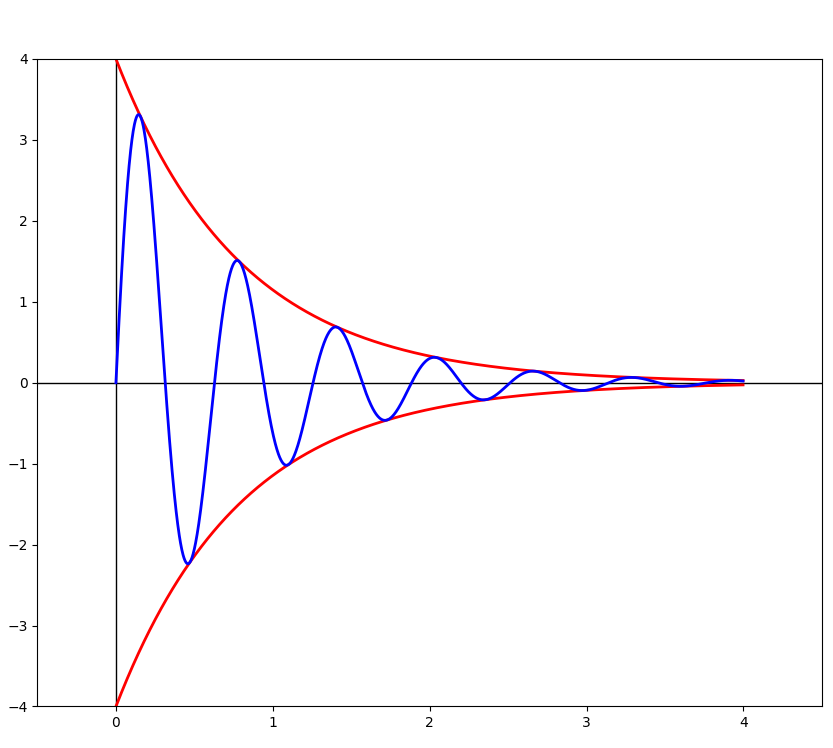
\includegraphics[scale=0.3625]{fig4.png}
	\caption{In blue: Graph of the solution when $c < \sqrt{4mk}$. In red: Graph of $\pm Re^{-ct/2m}$.}
	\end{figure}
	
	\newpage
	
	\subsection{Overdamped Motion}
	\begin{itemize}
	\item The system is said to be \textbf{overdamped} if $c > \sqrt{4mk}$. 
	\item The roots are 
		\begin{align*}
		r_1 = \frac{-c - \sqrt{c^2 - 4mk}}{2m} \text{ and } \quad r_2 = \frac{-c + \sqrt{c^2 - 4mk}}{2m} .
		\end{align*}
	We have $r_1 < r_2 < 0$.
	\item The general solution is
		\begin{align*}
		y(t) = c_1 e^{r_1 t} + c_2 e^{r_2 t} .
		\end{align*}
	\item We remark that $\lim_{t \ra \infty} y(t) = 0$.
	\end{itemize}
	
	\begin{figure}[h]
	\centering
	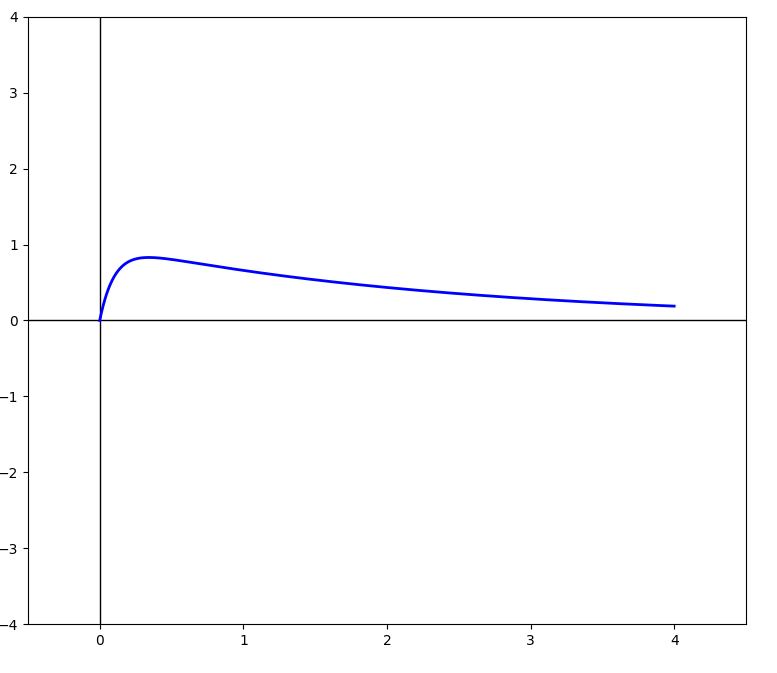
\includegraphics[scale=0.5]{fig5.png}
	\caption{Overdamped System}
	\end{figure}
	
	\newpage
	
	\subsection{Critically Damped Motion}
	
	\begin{itemize}
	\item The system is said to be \textbf{critically damped} if $c = \sqrt{4mk}$.
	\item The roots are
		\begin{align*}
		r_1 = r_2 = -\frac{c}{2m} .
		\end{align*}
	\item The general solution is therefore
		\begin{align*}
		y(t) = e^{-ct/2m} (c_1 + c_2 t) .
		\end{align*}
	\item We see that $\lim_{t \ra \infty} y(t) = 0$.
	\end{itemize}
	
	\begin{figure}[h]
	\centering
	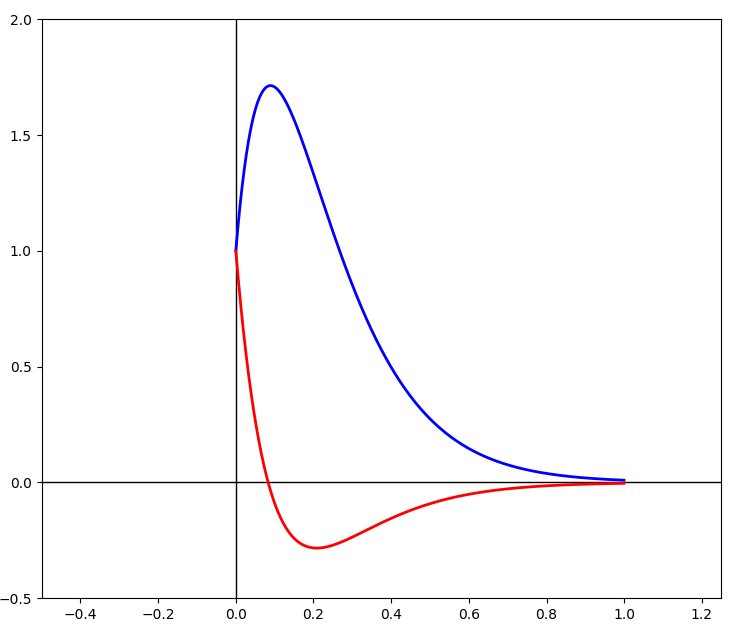
\includegraphics[scale=0.5]{fig6.png}
	\caption{In blue: $y(t) = e^{-8t}(1 + 28t)$. In red: $y(t) = e^{-8t} (1 - 12t)$.}
	\end{figure}

\end{document}